\documentclass{article}
\usepackage{graphicx} 
\usepackage{listings}

\begin{document}

\title{TCP File Transfer Protocol}
\author{Dinh Khanh Minh Bi12-154}
\date{\today}

\maketitle

\begin{abstract}
Task goal: Creating a simple file transfer protocol using TCP/IP sockets with C++. \newline 
The server: listens for incoming connections on a specified port + receives a file from client. \newline
The client then connects to the server -> sends the file contents.
\end{abstract}

\section{Initializing Programs}

\includegraphics[width=1\linewidth]{init.png}

\section{Protocol Design}

The protocol follows a basic request-response pattern:

\subsection{Client}

1. Using the designated port, connects to the server.\newline 
2. Recieve the name of the file to transfer.\newline 
3. Sends the file data in chunks.\newline 

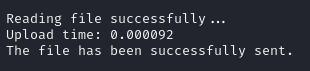
\includegraphics[width=1\linewidth]{client.png}
\subsection{Server}

1. Using the specified port, listens for incoming connections.\newline 
2. Accepts a client's connection.\newline 
3. Receives the filename from the client.\newline 
4. Receives the file data in chunks and writes it to a file on the server.\newline 

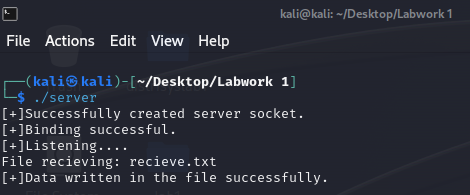
\includegraphics[width=1\linewidth]{server.png}

\section{System Organization}

There are two main components of the server:

\subsection{Server}

This program listens for incoming connections and receives files from clients.
\begin{lstlisting}[language=C++, caption=Sever C++ Code, label=lst:code]
#include <iostream>
#include <stdio.h>
#include <stdlib.h>
#include <unistd.h>
#include <string.h>
#include <sys/types.h>
#include <sys/socket.h>
#include <arpa/inet.h>
#include <netinet/in.h>
#include <fstream>
#include <cstring>

#define SIZE 900000 // size of buffer 

void write_file(int sockfd){
  int n;
  std::ofstream fp;
  std::string filename = "recieve.txt";
  std::cout << "File recieving: " << filename << std::endl;
  char buffer[SIZE];

  fp.open(filename);
  while (1) {
    n = recv(sockfd, buffer, SIZE, 0);
    if (n <= 0){
      break;
      return;
    }
    fp << buffer;
    std::memset(buffer, 0, SIZE);
  }
  return;
}

int main() // main function
{
  std::string ip = "127.0.0.1";
  int port = 8080; // port number
  int e;

  int sockfd, new_sock;
  struct sockaddr_in server_addr, new_addr;
  socklen_t addr_size;
  char buffer[SIZE];

  sockfd = socket(AF_INET, SOCK_STREAM, 0); // create socket
  if(sockfd < 0) {
    perror("[-]Socket error."); 
    exit(1);
  }
  std::cout << "[+]Successfully created server socket.\n";

  server_addr.sin_family = AF_INET;
  server_addr.sin_port = port;
  server_addr.sin_addr.s_addr = inet_addr(ip.c_str());

  e = bind(sockfd, (struct sockaddr*)&server_addr, sizeof(server_addr)); // bind the socket
  if(e < 0) {
    perror("[-]Bind error.");
    exit(1);
  }
  std::cout << "[+]Binding successful.\n";

  if(listen(sockfd, 10) == 0){ // listen for connection
    std::cout << "[+]Listening....\n";
  }else{
    perror("[-]Listening error.");
    exit(1);
  }

  addr_size = sizeof(new_addr); // accept the connection
  new_sock = accept(sockfd, (struct sockaddr*)&new_addr, &addr_size);
  write_file(new_sock);
  std::cout << "[+]Data written in the file successfully.\n";

  return 0;
}
\end{lstlisting}

\subsection{Client}

This program connects to the server, sends a filename, and transmits the file content.
\begin{lstlisting}[language=C++, caption=Client C++ Code, label=lst:code]
#include <iostream>
#include <stdio.h>
#include <stdlib.h>
#include <unistd.h>
#include <string.h>
#include <sys/types.h>
#include <sys/socket.h>
#include <arpa/inet.h>
#include <netinet/in.h>

#include <iostream>
#include <fstream>
#include <cstring>
#include <arpa/inet.h>
#define SIZE 99999

void send_file(std::ifstream& fp, int sockfd){
  int n;
  char data[SIZE] = {0};

  while(fp.getline(data, SIZE)) {
    if (send(sockfd, data, sizeof(data), 0) == -1) {
      perror("[-]File sending error.");
      exit(1);
    }
    std::memset(data, 0, SIZE);
  }
}

int main(){
  std::string ip = "127.0.0.1";
  int port = 8080;
  int e;

  int sockfd;
  struct sockaddr_in server_addr;
  std::ifstream fp;
  std::string filename;
  std::cout << "Enter filename to send: ";
  std::getline(std::cin, filename);

  sockfd = socket(AF_INET, SOCK_STREAM, 0);
  if(sockfd < 0) {
    perror("[-]Socket error.");
    exit(1);
  }
  std::cout << "[+]Successfully created server socket.\n";

  server_addr.sin_family = AF_INET;
  server_addr.sin_port = port;
  server_addr.sin_addr.s_addr = inet_addr(ip.c_str());

  e = connect(sockfd, (struct sockaddr*)&server_addr, sizeof(server_addr));
  if(e == -1) {
    perror("[-]Socket error");
    exit(1);
  }
  std::cout << "[+]Connected to Server.\n";
  std::cout << "Name of the file to send: ";
  std::getline(std::cin, filename);
  fp.open(filename);
  if (!fp) {
    perror("[-]File reading error.");
    exit(1);
  }

  send_file(fp, sockfd);
  std::cout << "[+]Successfully sent file data.\n";

  std::cout << "[+]Closing connection...\n";
  close(sockfd);

  return 0;
}
\end{lstlisting}
\begin{figure}
    \centering
    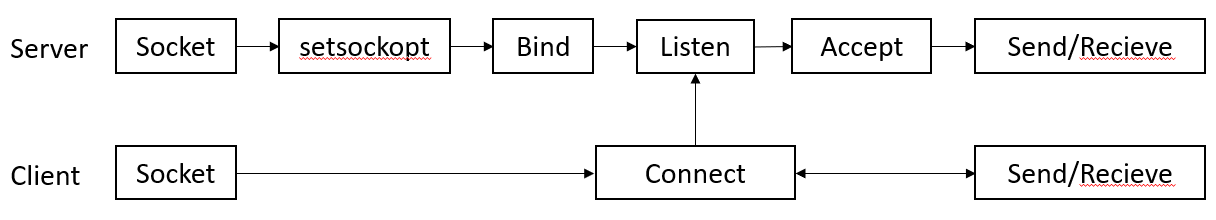
\includegraphics[width=1\linewidth]{socket_server_diagram.png}
    \caption{Figure 1. Flowchart of TCP file transfer}
    \label{fig:enter-label}
\end{figure}
\end{document}

